\documentclass{standalone}
\usepackage{tikz}
\usetikzlibrary{patterns, positioning}


\begin{document}
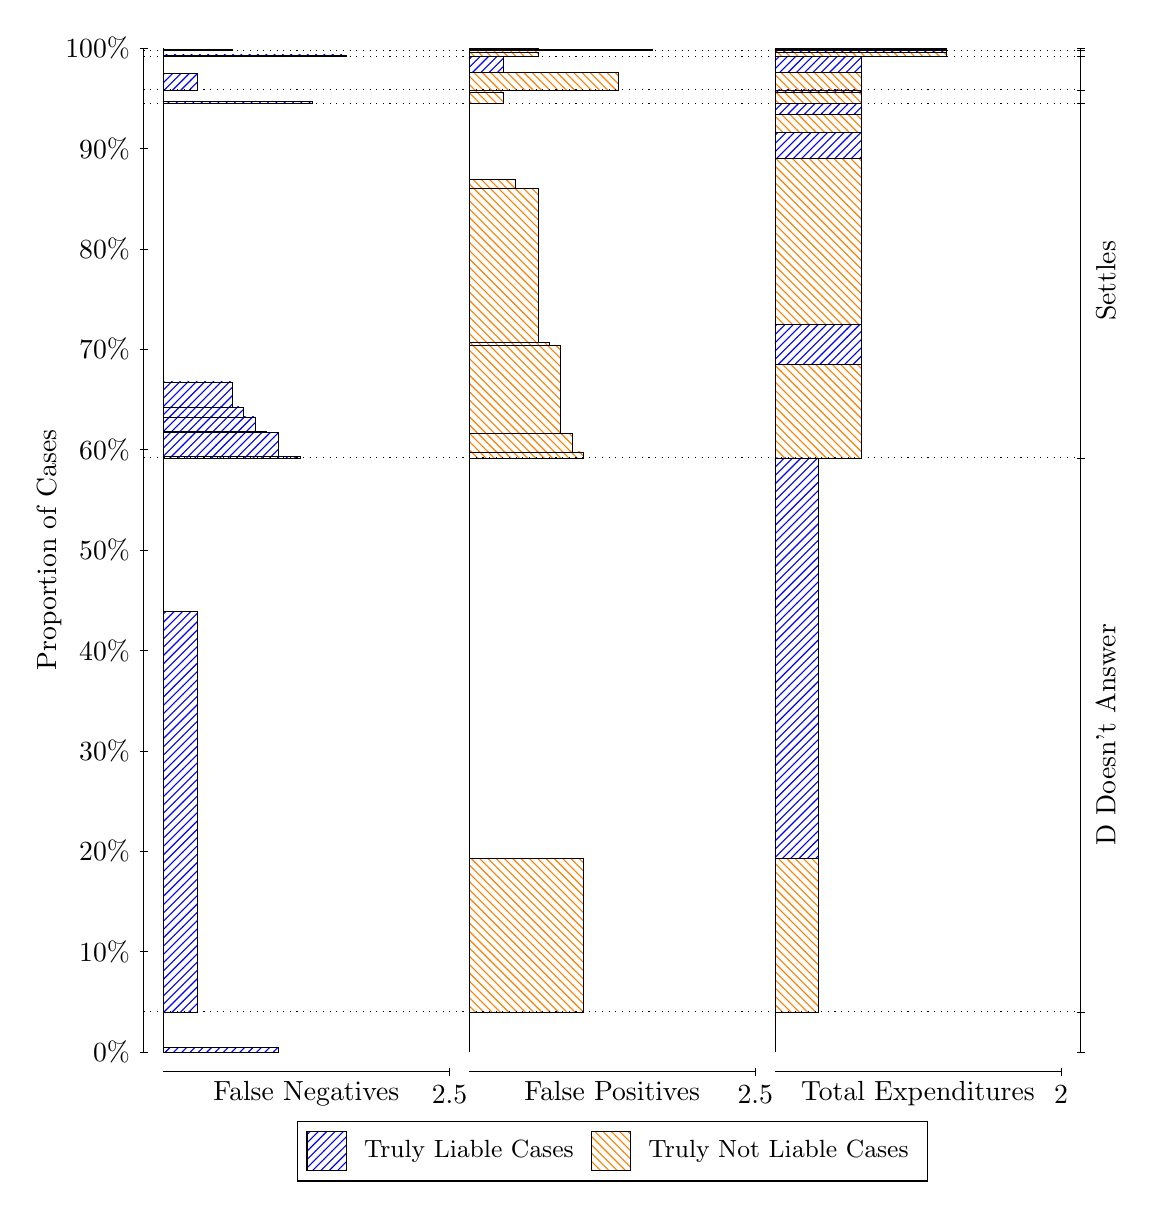
\begin{tikzpicture}
\draw[black, very thin] (1.5,1.75) -- (1.5,14.5);
\node[rotate=90, text=black, anchor=center] at (0.3, 8.125) {Proportion of Cases};
\draw[black, very thin] (1.45,1.75) -- (1.55,1.75);
\node[text=black, anchor=east] at (1.45, 1.75) {0\%};
\draw[black, very thin] (1.45,3.025) -- (1.55,3.025);
\node[text=black, anchor=east] at (1.45, 3.025) {10\%};
\draw[black, very thin] (1.45,4.3) -- (1.55,4.3);
\node[text=black, anchor=east] at (1.45, 4.3) {20\%};
\draw[black, very thin] (1.45,5.575) -- (1.55,5.575);
\node[text=black, anchor=east] at (1.45, 5.575) {30\%};
\draw[black, very thin] (1.45,6.85) -- (1.55,6.85);
\node[text=black, anchor=east] at (1.45, 6.85) {40\%};
\draw[black, very thin] (1.45,8.125) -- (1.55,8.125);
\node[text=black, anchor=east] at (1.45, 8.125) {50\%};
\draw[black, very thin] (1.45,9.4) -- (1.55,9.4);
\node[text=black, anchor=east] at (1.45, 9.4) {60\%};
\draw[black, very thin] (1.45,10.675) -- (1.55,10.675);
\node[text=black, anchor=east] at (1.45, 10.675) {70\%};
\draw[black, very thin] (1.45,11.95) -- (1.55,11.95);
\node[text=black, anchor=east] at (1.45, 11.95) {80\%};
\draw[black, very thin] (1.45,13.225) -- (1.55,13.225);
\node[text=black, anchor=east] at (1.45, 13.225) {90\%};
\draw[black, very thin] (1.45,14.5) -- (1.55,14.5);
\node[text=black, anchor=east] at (1.45, 14.5) {100\%};

\draw[black, very thin] (13.4,1.75) -- (13.4,14.5);
\draw[black, very thin] (13.35,1.75) -- (13.45,1.75);
\node[anchor=west] at (13.35, 1.75) {};
\draw[black, very thin] (13.35,2.2584) -- (13.45,2.2584);
\node[anchor=west] at (13.35, 2.2584) {};
\draw[black, very thin] (13.35,9.2942) -- (13.45,9.2942);
\node[anchor=west] at (13.35, 9.2942) {};
\draw[black, very thin] (13.35,13.792) -- (13.45,13.792);
\node[anchor=west] at (13.35, 13.792) {};
\draw[black, very thin] (13.35,13.969) -- (13.45,13.969);
\node[anchor=west] at (13.35, 13.969) {};
\draw[black, very thin] (13.35,14.396) -- (13.45,14.396);
\node[anchor=west] at (13.35, 14.396) {};
\draw[black, very thin] (13.35,14.468) -- (13.45,14.468);
\node[anchor=west] at (13.35, 14.468) {};
\draw[black, very thin] (13.35,14.5) -- (13.45,14.5);
\node[anchor=west] at (13.35, 14.5) {};

\draw[black, very thin, pattern color=blue, pattern=north east lines] (1.75,1.75) rectangle (3.2033,1.8035);
\draw[black, very thin, pattern color=orange, pattern=north west lines] (1.75,1.8035) rectangle (1.75,2.2584);
\draw[black, very thin, pattern color=blue, pattern=north east lines] (1.75,2.2584) rectangle (2.186,7.3487);
\draw[black, very thin, pattern color=orange, pattern=north west lines] (1.75,7.3487) rectangle (1.75,9.2942);
\draw[black, very thin, pattern color=blue, pattern=north east lines] (1.75,9.2942) rectangle (3.494,9.3121);
\draw[black, very thin, pattern color=blue, pattern=north east lines] (1.75,9.3121) rectangle (3.2033,9.6159);
\draw[black, very thin, pattern color=blue, pattern=north east lines] (1.75,9.6159) rectangle (3.058,9.628);
\draw[black, very thin, pattern color=blue, pattern=north east lines] (1.75,9.628) rectangle (2.9127,9.8143);
\draw[black, very thin, pattern color=blue, pattern=north east lines] (1.75,9.8143) rectangle (2.7673,9.9421);
\draw[black, very thin, pattern color=blue, pattern=north east lines] (1.75,9.9421) rectangle (2.622,10.259);
\draw[black, very thin, pattern color=orange, pattern=north west lines] (1.75,10.259) rectangle (1.75,13.792);
\draw[black, very thin, pattern color=blue, pattern=north east lines] (1.75,13.792) rectangle (3.6393,13.818);
\draw[black, very thin, pattern color=orange, pattern=north west lines] (1.75,13.818) rectangle (1.75,13.969);
\draw[black, very thin, pattern color=blue, pattern=north east lines] (1.75,13.969) rectangle (2.186,14.178);
\draw[black, very thin, pattern color=orange, pattern=north west lines] (1.75,14.178) rectangle (1.75,14.396);
\draw[black, very thin, pattern color=blue, pattern=north east lines] (1.75,14.396) rectangle (4.0753,14.412);
\draw[black, very thin, pattern color=orange, pattern=north west lines] (1.75,14.412) rectangle (1.75,14.468);
\draw[black, very thin, pattern color=blue, pattern=north east lines] (1.75,14.468) rectangle (2.622,14.484);
\draw[black, very thin, pattern color=orange, pattern=north west lines] (1.75,14.484) rectangle (1.75,14.5);
\draw[black, very thin, pattern color=orange, pattern=north west lines] (5.6333,1.75) rectangle (5.6333,2.2049);
\draw[black, very thin, pattern color=blue, pattern=north east lines] (5.6333,2.2049) rectangle (5.6333,2.2584);
\draw[black, very thin, pattern color=orange, pattern=north west lines] (5.6333,2.2584) rectangle (7.0867,4.2038);
\draw[black, very thin, pattern color=blue, pattern=north east lines] (5.6333,4.2038) rectangle (5.6333,9.2942);
\draw[black, very thin, pattern color=orange, pattern=north west lines] (5.6333,9.2942) rectangle (7.0867,9.3716);
\draw[black, very thin, pattern color=orange, pattern=north west lines] (5.6333,9.3716) rectangle (6.9413,9.6083);
\draw[black, very thin, pattern color=orange, pattern=north west lines] (5.6333,9.6083) rectangle (6.796,10.722);
\draw[black, very thin, pattern color=orange, pattern=north west lines] (5.6333,10.722) rectangle (6.6507,10.766);
\draw[black, very thin, pattern color=orange, pattern=north west lines] (5.6333,10.766) rectangle (6.5053,12.716);
\draw[black, very thin, pattern color=orange, pattern=north west lines] (5.6333,12.716) rectangle (6.2147,12.828);
\draw[black, very thin, pattern color=blue, pattern=north east lines] (5.6333,12.828) rectangle (5.6333,13.792);
\draw[black, very thin, pattern color=orange, pattern=north west lines] (5.6333,13.792) rectangle (6.0693,13.944);
\draw[black, very thin, pattern color=blue, pattern=north east lines] (5.6333,13.944) rectangle (5.6333,13.969);
\draw[black, very thin, pattern color=orange, pattern=north west lines] (5.6333,13.969) rectangle (7.5227,14.187);
\draw[black, very thin, pattern color=blue, pattern=north east lines] (5.6333,14.187) rectangle (6.0693,14.396);
\draw[black, very thin, pattern color=orange, pattern=north west lines] (5.6333,14.396) rectangle (6.5053,14.452);
\draw[black, very thin, pattern color=blue, pattern=north east lines] (5.6333,14.452) rectangle (5.6333,14.468);
\draw[black, very thin, pattern color=orange, pattern=north west lines] (5.6333,14.468) rectangle (7.9587,14.484);
\draw[black, very thin, pattern color=blue, pattern=north east lines] (5.6333,14.484) rectangle (6.5053,14.5);
\draw[black, very thin, pattern color=orange, pattern=north west lines] (9.5167,1.75) rectangle (9.5167,2.2049);
\draw[black, very thin, pattern color=blue, pattern=north east lines] (9.5167,2.2049) rectangle (9.5167,2.2584);
\draw[black, very thin, pattern color=orange, pattern=north west lines] (9.5167,2.2584) rectangle (10.062,4.2038);
\draw[black, very thin, pattern color=blue, pattern=north east lines] (9.5167,4.2038) rectangle (10.062,9.2942);
\draw[black, very thin, pattern color=orange, pattern=north west lines] (9.5167,9.2942) rectangle (10.607,10.485);
\draw[black, very thin, pattern color=blue, pattern=north east lines] (9.5167,10.485) rectangle (10.607,10.988);
\draw[black, very thin, pattern color=orange, pattern=north west lines] (9.5167,10.988) rectangle (10.607,13.094);
\draw[black, very thin, pattern color=blue, pattern=north east lines] (9.5167,13.094) rectangle (10.607,13.428);
\draw[black, very thin, pattern color=orange, pattern=north west lines] (9.5167,13.428) rectangle (10.607,13.665);
\draw[black, very thin, pattern color=blue, pattern=north east lines] (9.5167,13.665) rectangle (10.607,13.792);
\draw[black, very thin, pattern color=orange, pattern=north west lines] (9.5167,13.792) rectangle (10.607,13.944);
\draw[black, very thin, pattern color=blue, pattern=north east lines] (9.5167,13.944) rectangle (10.607,13.969);
\draw[black, very thin, pattern color=orange, pattern=north west lines] (9.5167,13.969) rectangle (10.607,14.187);
\draw[black, very thin, pattern color=blue, pattern=north east lines] (9.5167,14.187) rectangle (10.607,14.396);
\draw[black, very thin, pattern color=orange, pattern=north west lines] (9.5167,14.396) rectangle (11.697,14.452);
\draw[black, very thin, pattern color=blue, pattern=north east lines] (9.5167,14.452) rectangle (11.697,14.468);
\draw[black, very thin, pattern color=orange, pattern=north west lines] (9.5167,14.468) rectangle (11.697,14.484);
\draw[black, very thin, pattern color=blue, pattern=north east lines] (9.5167,14.484) rectangle (11.697,14.5);
\draw[black, dotted] (1.5,2.2584) -- (13.4,2.2584);
\draw[black, dotted] (1.5,9.2942) -- (13.4,9.2942);
\draw[black, dotted] (1.5,13.792) -- (13.4,13.792);
\draw[black, dotted] (1.5,13.969) -- (13.4,13.969);
\draw[black, dotted] (1.5,14.396) -- (13.4,14.396);
\draw[black, dotted] (1.5,14.468) -- (13.4,14.468);
\draw[black, very thin] (1.75,1.5) -- (5.3833,1.5);
\node[text=black, anchor=north] at (3.5667, 1.5) {False Negatives};
\draw[black, very thin] (5.3833,1.45) -- (5.3833,1.55);
\node[text=black, anchor=north] at (5.3833, 1.45) {2.5};

\draw[black, very thin] (5.6333,1.5) -- (9.2667,1.5);
\node[text=black, anchor=north] at (7.45, 1.5) {False Positives};
\draw[black, very thin] (9.2667,1.45) -- (9.2667,1.55);
\node[text=black, anchor=north] at (9.2667, 1.45) {2.5};

\draw[black, very thin] (9.5167,1.5) -- (13.15,1.5);
\node[text=black, anchor=north] at (11.333, 1.5) {Total Expenditures};
\draw[black, very thin] (13.15,1.45) -- (13.15,1.55);
\node[text=black, anchor=north] at (13.15, 1.45) {2};


\node[text=black, centered, rotate=90] at (13.72, 5.7763) {D Doesn't Answer};
\node[text=black, centered, rotate=90] at (13.72, 11.543) {Settles};





\draw (7.449999999999999,1.5) node[draw=none] (baseCoordinate) {};
\begin{scope}[align=center]
        \matrix[scale=0.5, draw=black, below=0.5cm of baseCoordinate, nodes={draw}, column sep=0.1cm]{
            \node[rectangle, draw, minimum width=0.5cm, minimum height=0.5cm, pattern color=blue, pattern=north east lines] {}; &
            \node[draw=none, font=\small, text=black] (B) {Truly Liable Cases}; &
            \node[rectangle, draw, minimum width=0.5cm, minimum height=0.5cm, pattern color=orange, pattern=north west lines] {}; &
            \node[draw=none, font=\small, text=black] (B) {Truly Not Liable Cases}; \\
            };
\end{scope}

\end{tikzpicture}
\end{document}